\section{PERFORM: Open-source ROM Development}

Before describing the one-dimensional premixed flame model which we will examine in this chapter, we highlight the Prototyping Environment for Reaction Flow Order Reduction Methods (PERFORM)~\cite{Wentland2022}, an open-source Python package developed for the purpose of studying ROMs for simple reacting flows. This work was motivated by a general dearth of research on ROMs for reacting flows, which may be attributed to the complexity of reacting flow modeling combined with a lack of approachable open-source libraries for combustion CFD. Originally developed for internal use by collaborators, PERFORM is equipped with a self-contained one-dimensional, compressible reacting flow solver which may be queried by a separate ROM framework which is designed for code flexibility and expansion. The package thus serves as a general-purpose testbed for novel ROM methods in both its capacity to generate challenging datasets for non-intrusive approaches, as well its expressive construction which allows for rapid implementation of novel intrusive approaches.  In this sense, PERFORM lowers the barrier to entry for ROM researchers who may have little experience with combustion modeling or low-level programming languages, allowing them to perform research with a challenging, practical class of problems.

We briefly describe PERFORM's structure, which is very roughly visualized in Fig.~\ref{fig:performAPI}. As mentioned previously, the 1D finite-volume flow solver and ROM framework are purposely segregated such that ROM method developers do not need to interact with the flow solver beyond querying functions which calculate, e.g., $\rhsFunc{\cdot}$, $\resFunc{\cdot}$. The flow solver, packaged under the class \texttt{SolutionDomain}, contains generic interfaces for the standard trappings of any finite volume flow solver, including gas models (\texttt{GasModel}), chemical reaction models (\texttt{ReactionModel}), fluxes (\texttt{Flux}), temporal integrators (\texttt{TimeIntegrator}), gradient limiters (\texttt{Limiter}), and \textit{in situ} data visualizations (\texttt{Visualization}). These interfaces are easily expanded beyond PERFORM's current offerings thanks to judicious use of Python's class inheritance and polymorphism.

\begin{figure}
	\begin{minipage}{0.49\linewidth}
		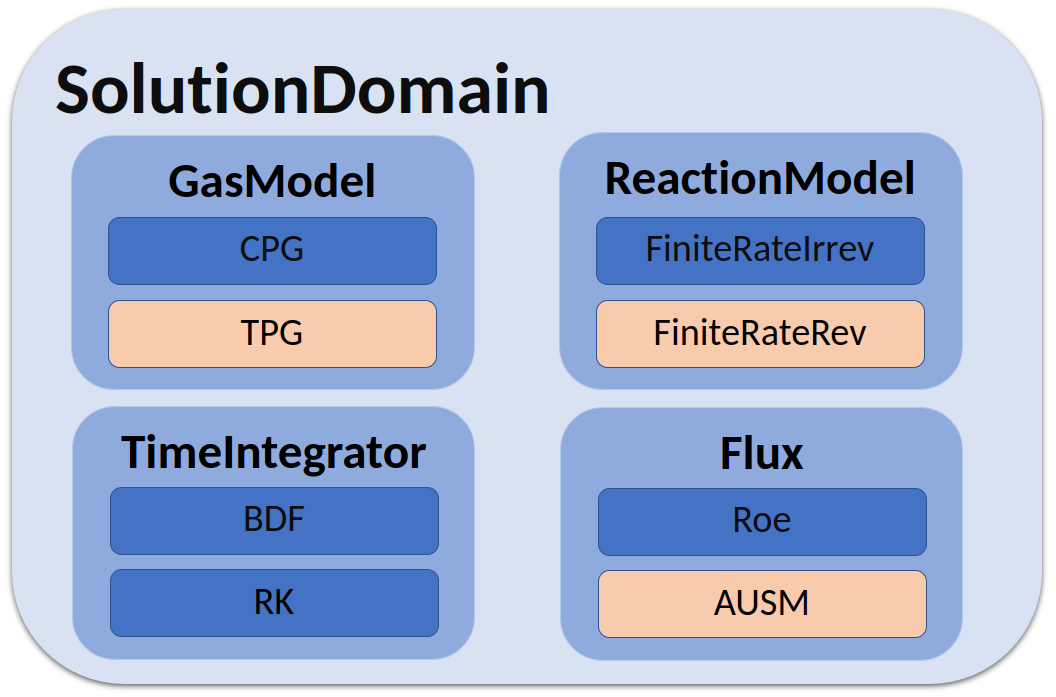
\includegraphics[width=0.99\linewidth]{Chapters/TransientFlame/Images/performFOMAPI.png}
	\end{minipage}
	\begin{minipage}{0.49\linewidth}
		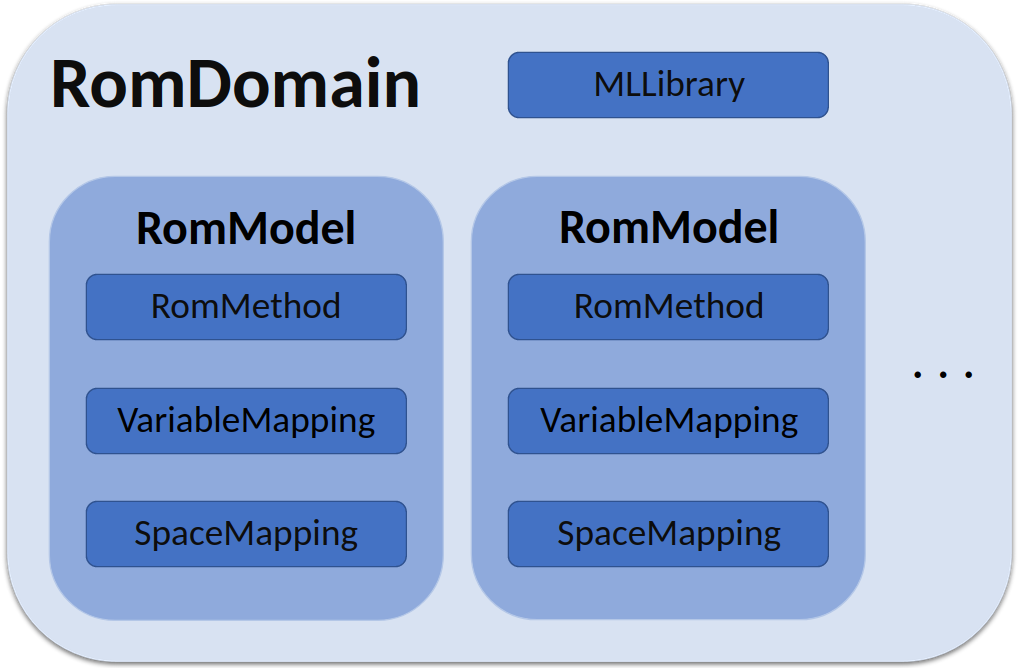
\includegraphics[width=0.99\linewidth]{Chapters/TransientFlame/Images/performROMAPI.png}
	\end{minipage}
	\caption{\label{fig:performAPI}Simplified PERFORM class hierarchy for flow solver (left) and ROM solver (right). Class instances in blue have been implemented, those in orange are under development.}
\end{figure}

The overarching reduced-order model solver class, \texttt{RomDomain}, is designed to provide maximum flexibility to ROM developers. A given ROM solve may be decomposed into several self-contained \texttt{RomModel}s, which govern how the low dimensional representation for a subset of flow variables is evolved in time. For example, one model might target pressure and velocity, while another might target temperature and species mass fractions (linked to the ``scalar'' ROM concept explored by Zhou~\cite{Zhou2012}). Generic interfaces for specifying target variables (\texttt{RomVariableMapping}), defining mappings from the latent space to the trial manifold (\texttt{RomSpaceMapping}), and specifying non-standard time evolution methods (\texttt{RomTimeStepper}) are similarly simple to expand to meet development needs. Generic interfaces to machine learning libraries such as TensorFlow are also provided.

PERFORM is available as a public repository\footnote{https://github.com/cwentland0/perform}, and comes with several benchmark cases which are ready to run out-of-the-box. These cases include a Sod shock tube, a transient multi-species contact surface (with and without artificial acoustic forcing), a stationary premixed flame (with artificial acoustic forcing), and a transient premixed flame (with and without artificial acoustic forcing). This last case will be analyzed in the following sections. The benchmarks address several of the critical issues facing the broader ROM community, particularly the difficulty of propagating transient flow features beyond the training data set and making accurate predictions in a complex parameter space. The code has already seen successful use in developing accurate and robust linearized ROMs~\cite{Rezaian2022} and investigating true ROM predictivity via basis and hyper-reduction sampling adaptation~\cite{WayneIsaacTanUy2022}.